\documentclass[journal,12pt,twocolumn]{IEEEtran}
\usepackage{amsthm}
\allowbreak
\usepackage{setspace}
\usepackage{gensymb}
\singlespacing
\usepackage[cmex10]{amsmath}
\usepackage{caption}
\usepackage{amsthm}



\DeclareUnicodeCharacter{2212}{-}
\usepackage{tikz}
\usepackage{pgfplots}

\usepackage{mathrsfs}
\usepackage{txfonts}
\usepackage{stfloats}
\usepackage{bm}
\usepackage{cite}
\usepackage{cases}
\usepackage{subfig}

\usepackage{longtable}
\usepackage{multirow}

\usepackage{enumitem}
\usepackage{mathtools}
\usepackage{steinmetz}
\usepackage{tikz}
\usepackage{circuitikz}
\usepackage{verbatim}
\usepackage{tfrupee}
\usepackage[breaklinks=true]{hyperref}
\usepackage{graphicx}
\usepackage{tkz-euclide}
\graphicspath{ {./images/} }
\usetikzlibrary{calc,math}
\usepackage{listings}
    \usepackage{color}                                            %%
    \usepackage{array}                                            %%
    \usepackage{longtable}                                        %%
    \usepackage{calc}                                             %%
    \usepackage{multirow}                                         %%
    \usepackage{hhline}                                           %%
    \usepackage{ifthen}                                           %%
    \usepackage{lscape}     
\usepackage{multicol}
\usepackage{chngcntr}

\DeclareMathOperator*{\Res}{Res}

\renewcommand\thesection{\arabic{section}}
\renewcommand\thesubsection{\thesection.\arabic{subsection}}
\renewcommand\thesubsubsection{\thesubsection.\arabic{subsubsection}}

\renewcommand\thesectiondis{\arabic{section}}
\renewcommand\thesubsectiondis{\thesectiondis.\arabic{subsection}}
\renewcommand\thesubsubsectiondis{\thesubsectiondis.\arabic{subsubsection}}


\hyphenation{op-tical net-works semi-conduc-tor}
\def\inputGnumericTable{}                                 %%

\lstset{
%language=C,
frame=single, 
breaklines=true,
columns=fullflexible
}
\begin{document}


\newtheorem{theorem}{Theorem}[section]
\newtheorem{problem}{Problem}
\newtheorem{proposition}{Proposition}[section]
\newtheorem{lemma}{Lemma}[section]
\newtheorem{corollary}[theorem]{Corollary}
\newtheorem{example}{Example}[section]
\newtheorem{definition}[problem]{Definition}

\newcommand{\BEQA}{\begin{eqnarray}}
\newcommand{\EEQA}{\end{eqnarray}}
\newcommand{\define}{\stackrel{\triangle}{=}}
\bibliographystyle{IEEEtran}
\raggedbottom
\setlength{\parindent}{0pt}
\providecommand{\mbf}{\mathbf}
\providecommand{\pr}[1]{\ensuremath{\Pr\left(#1\right)}}
\providecommand{\qfunc}[1]{\ensuremath{Q\left(#1\right)}}
\providecommand{\sbrak}[1]{\ensuremath{{}\left[#1\right]}}
\providecommand{\lsbrak}[1]{\ensuremath{{}\left[#1\right.}}
\providecommand{\rsbrak}[1]{\ensuremath{{}\left.#1\right]}}
\providecommand{\brak}[1]{\ensuremath{\left(#1\right)}}
\providecommand{\lbrak}[1]{\ensuremath{\left(#1\right.}}
\providecommand{\rbrak}[1]{\ensuremath{\left.#1\right)}}
\providecommand{\cbrak}[1]{\ensuremath{\left\{#1\right\}}}
\providecommand{\lcbrak}[1]{\ensuremath{\left\{#1\right.}}
\providecommand{\rcbrak}[1]{\ensuremath{\left.#1\right\}}}
\theoremstyle{remark}
\newtheorem{rem}{Remark}
\newcommand{\sgn}{\mathop{\mathrm{sgn}}}
\providecommand{\abs}[1]{$\left\vert#1\right\vert$}
\providecommand{\res}[1]{\Res\displaylimits_{#1}} 
\providecommand{\norm}[1]{$\left\lVert#1\right\rVert$}
%\providecommand{\norm}[1]{\lVert#1\rVert}
\providecommand{\mtx}[1]{\mathbf{#1}}
\providecommand{\mean}[1]{E$\left[ #1 \right]$}
\providecommand{\fourier}{\overset{\mathcal{F}}{ \rightleftharpoons}}
%\providecommand{\hilbert}{\overset{\mathcal{H}}{ \rightleftharpoons}}
\providecommand{\system}{\overset{\mathcal{H}}{ \longleftrightarrow}}
	%\newcommand{\solution}[2]{\textbf{Solution:}{#1}}
\newcommand{\solution}{\noindent \textbf{Solution: }}
\newcommand{\cosec}{\,\text{cosec}\,}
\providecommand{\dec}[2]{\ensuremath{\overset{#1}{\underset{#2}{\gtrless}}}}
\newcommand{\myvec}[1]{\ensuremath{\begin{pmatrix}#1\end{pmatrix}}}
\newcommand{\mydet}[1]{\ensuremath{\begin{vmatrix}#1\end{vmatrix}}}
\numberwithin{equation}{subsection}
\makeatletter
\@addtoreset{figure}{problem}
\makeatother
\let\StandardTheFigure\thefigure
\let\vec\mathbf
\renewcommand{\thefigure}{\theproblem}
\def\putbox#1#2#3{\makebox[0in][l]{\makebox[#1][l]{}\raisebox{\baselineskip}[0in][0in]{\raisebox{#2}[0in][0in]{#3}}}}
     \def\rightbox#1{\makebox[0in][r]{#1}}
     \def\centbox#1{\makebox[0in]{#1}}
     \def\topbox#1{\raisebox{-\baselineskip}[0in][0in]{#1}}
     \def\midbox#1{\raisebox{-0.5\baselineskip}[0in][0in]{#1}}
\vspace{3cm}
\title{AI1103: Assignment 7}
\author{Tanmay Garg \\CS20BTECH11063 EE20BTECH11048}
\maketitle
\newpage
\bigskip
\renewcommand{\thefigure}{\theenumi}
\renewcommand{\thetable}{\theenumi}
Download all python codes from 
\begin{lstlisting}
https://github.com/tanmaygar/AI-Course/blob/main/Assignment7/Codes/CSIRUGC_NET%20EXAM_(Dec%202016)_Q51.py
\end{lstlisting}
%
and latex-tikz codes from 
%
\begin{lstlisting}
https://github.com/tanmaygar/AI-Course/blob/main/Assignment7/Assignment7.tex
\end{lstlisting}
\section*{Problem CSIR UGC NET EXAM (Dec 2016), Q.51: }
Suppose customers arrive in a shop according to a Poisson process with rate $4$ per hour. The shop opens at $10:00$ am. If it is given that the second customer arrives at $10:40 $ am, what is the probability that no customer arrived before $10:30 $ am? 
\begin{multicols}{4}
    \begin{enumerate}
        \item $\frac{1}{4}$
        \item $e^{-2}$
        \item $\frac{1}{2}$
        \item $e^{\frac{1}{2}}$
    \end{enumerate}
\end{multicols}
\section*{Solution:}
Let $X$ denote the random variable for the time interval, and it is divided as:
\begin{align*}
    p &= 10:00 - 10:30\\
    q &= 10:30 - 10:40\\
    r &= 10:00 - 10:40
\end{align*}
At the instant of $10:40$, let the random variable be $Y$.
We need to find
\begin{align}
    \pr{X_p = 0 | Y = 2} \label{main_eq}
\end{align}
In the world where the $2^{nd}$ person arrives at $10:40$ am the \eqref{main_eq} becomes:
\begin{align}
    &=\frac{\pr{X_p = 0, X_q = 1}}{\pr{X_r = 1}}\\
    &= \frac{\pr{X_p = 0} \times \pr{X_q = 1}}{\pr{X_r = 1}}\label{sub_eq}
\end{align}
The Poisson function distribution for time interval $t$ and rate $\lambda$ for a random variable $X$:
\[
    f_X(x,t) = \frac{(\lambda t)^x \exp{(-\lambda t)}}{x!}
\]
For the time interval $p$:
\begin{align}
    \lambda = 4, t &= 0.5, x= 0\\
    \pr{X_p = 0} &= f_X(0,0.5)\\
    &= e^{-2}\label{eq_1}
\end{align}
For the time interval $q$:
\begin{align}
    \lambda = 4, t &= \frac{1}{6},x = 1\\
    \pr{X_q = 1} &= f_X(1, \frac{1}{6})\\
    &= \frac{2}{3}e^{\frac{-2}{3}} \label{eq_2}
\end{align}
For the time interval $r$:
\begin{align}
    \lambda = 4, t &= \frac{2}{3}, x = 1\\
    \pr{X_r = 1} &= f_X(1, \frac{2}{3})\\
    &= \frac{8}{3}e^{\frac{-8}{3}} \label{eq_3}
\end{align}
Substituting \eqref{eq_1} \eqref{eq_2} \eqref{eq_3} in \eqref{sub_eq}:
\begin{align}
    \pr{X_p = 0 | Y = 2} = \frac{1}{4}
\end{align}
Hence, \textbf{Option 1} is correct\\
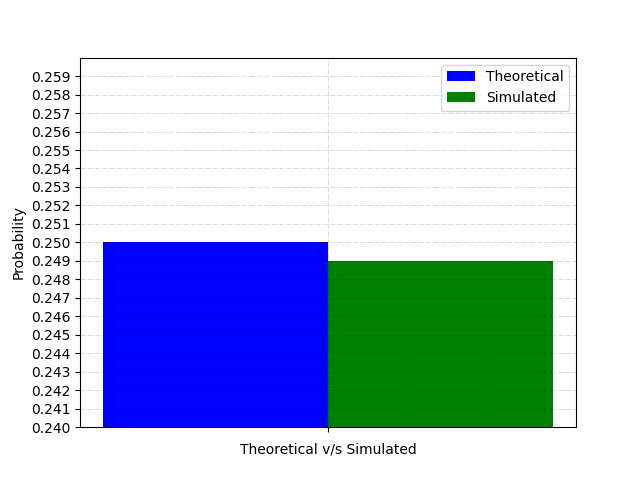
\includegraphics[width=\columnwidth]{Figure_4.png}
\end{document}